\chapter{State-of-the-Art}
\label{sec:state-of-the-art}

Since the release of the issue 1 standard, several implementations for hardware have been developed. Due to the lossless operation of the algorithm, image samples are used in place of the sample representatives of issue 2. This allows samples of different bands to be processed in parallel execution pipelines, an approach used by \citeauthor{orlandicParallelFPGAImplementation2019} to achieve a throughput of 750 MS/s \cite{orlandicParallelFPGAImplementation2019}. Samples are processed in the \acrshort{BIP} ordering, where image pixels are processed sequentially. Groups of $N_p$ samples are split according to their band and processed by $N_p$ pipelined cores. A different approach is used by \citeauthor{tsigkanosHighPerformanceCOTSFPGA2020}, in which images are split into segments that are compressed using separate, simpler cores. Using five parallel cores, a throughput of 1387 MS/s is reached.

Both of the mentioned issue 1 implementations support on-the-fly (real-time) processing, in which samples are processed immediately as they are made available from the image sensor. This is a desirable feature that reduces the need for temporary data storage. For the \acrshort{hypso}-1 image sensor, the real-time processing requirement is about 110.6 MS/s when operating at its maximum capacity of 47 frames per second with frames of size $1936x1216$ samples \cite{grotteOceanColorHyperspectral2022}. The real-time requirement differs between sensors, with the sensors of AVIRIS-NG and CHIME residing at 37.5 MS/s and 125 MS/s respectively \footnote{add cite to 18 and 21 from Bascones paper}[].

The quantization step, and subsequent sample representatives, of issue 2 introduce data dependencies in the predictor stage (\autoref{fig:dependencies}) that pose a challenge for pipelined hardware implementations. Parallel processing of samples using the method of \citeauthor{orlandicParallelFPGAImplementation2019} is no longer possible. \citeauthor{barriosHardwareImplementationCCSDS2021} present the first implementation of issue 2 in open literature, and is fully compliant with the standard \cite{barriosHardwareImplementationCCSDS2021}. Using the \acrshort{HLS} design methodology, they reach a low throughput of 18 MS/s. No special considerations as to the data dependencies are made, resulting in an almost fully serial implementation. This shows that a different approach is required to reach real-time operation. For the keen reader, a detailed of summary of key design specs of the following issue 2 implementations is presented in \autoref{tab:throughputs}. The table will also be discussed at the end of the chapter.

\begin{table}[ht]
	\caption{The number of processed samples interleaving $z-1$ and $t-1$ dependencies, including the novel FID ordering in addition to the standard orderings.}
	\label{tab:orderings-fid}
	\begin{center}
		\begin{tabular}{l l l l l l}
			\hline
			      & \textbf{BSQ}    & \textbf{BIP} & \textbf{BIL} & \textbf{FID} \\
			\hline
			$z-1$ & $N_x \cdot N_y$ & $1$          & $N_x$        & $N_z - 1$    \\
			$t-1$ & $1$             & $N_z$        & $1$          & $N_z$        \\
			\hline
		\end{tabular}
	\end{center}
\end{table}

As shown in \autoref{sec:compression}, data dependencies may be selectively bypassed by carefully selecting the sample processing order. This interleaves data dependant calculations by a number of other samples, allowing time for the dependency to resolve. The first viable real-time implementation of issue 2 is presented by \citeauthor{basconesFPGAAcceleratorRealTime2020}. By use of a novel sample processing order, dubbed \acrfull{FID}, they reach a throughput of 285 MS/s. \autoref{fig:fid} shows a visualization of the \acrshort{FID} processing order, with processed samples marked in white. Frames are concatenated along the $x$ dimension and processed diagonally, iterating on the $z$ and $x$ dimensions. The number of samples that interleave data dependencies can be obtained by counting along the diagonal, giving $N_z-1$ and $N_z$ samples for $z-1$ and $t-1$ dependencies respectively. This facilitates the deep pipeline of $57$ stages used by the implementation while allowing support for full and reduced prediction modes and all local sum types. Dependency interleaving of the different processing orders, including \acrshort{FID} is summarized in \autoref{tab:orderings-fid}.

The use of a new processing ordering requires reordering buffers that convert from the standard \acrshort{BIP} ordering. These are placed at each side of the predictor. The hybrid encoder module proceeds in \acrshort{BIP} ordering to result in a compressed bitstream compliant with the standard. Additionally, this allows integration into existing systems. The reordering buffers come at the cost of extra hardware resources, resulting in a somewhat larger footprint than that of \citeauthor{barriosHardwareImplementationCCSDS2021}. Especially in terms of \acrshort{BRAM}, which is increased from $85$ to $213$ due to storage required by the reordering buffers. Resource utilization is somewhat mitigated by use of portable \acrshort{RTL} written in VHDL, as opposed to the \acrshort{HLS} approach used by \citeauthor{barriosHardwareImplementationCCSDS2021}. Both implementations support runtime reconfiguration, adding additional hardware to provide flexibility.

\begin{figure}[ht]
	\begin{center}
		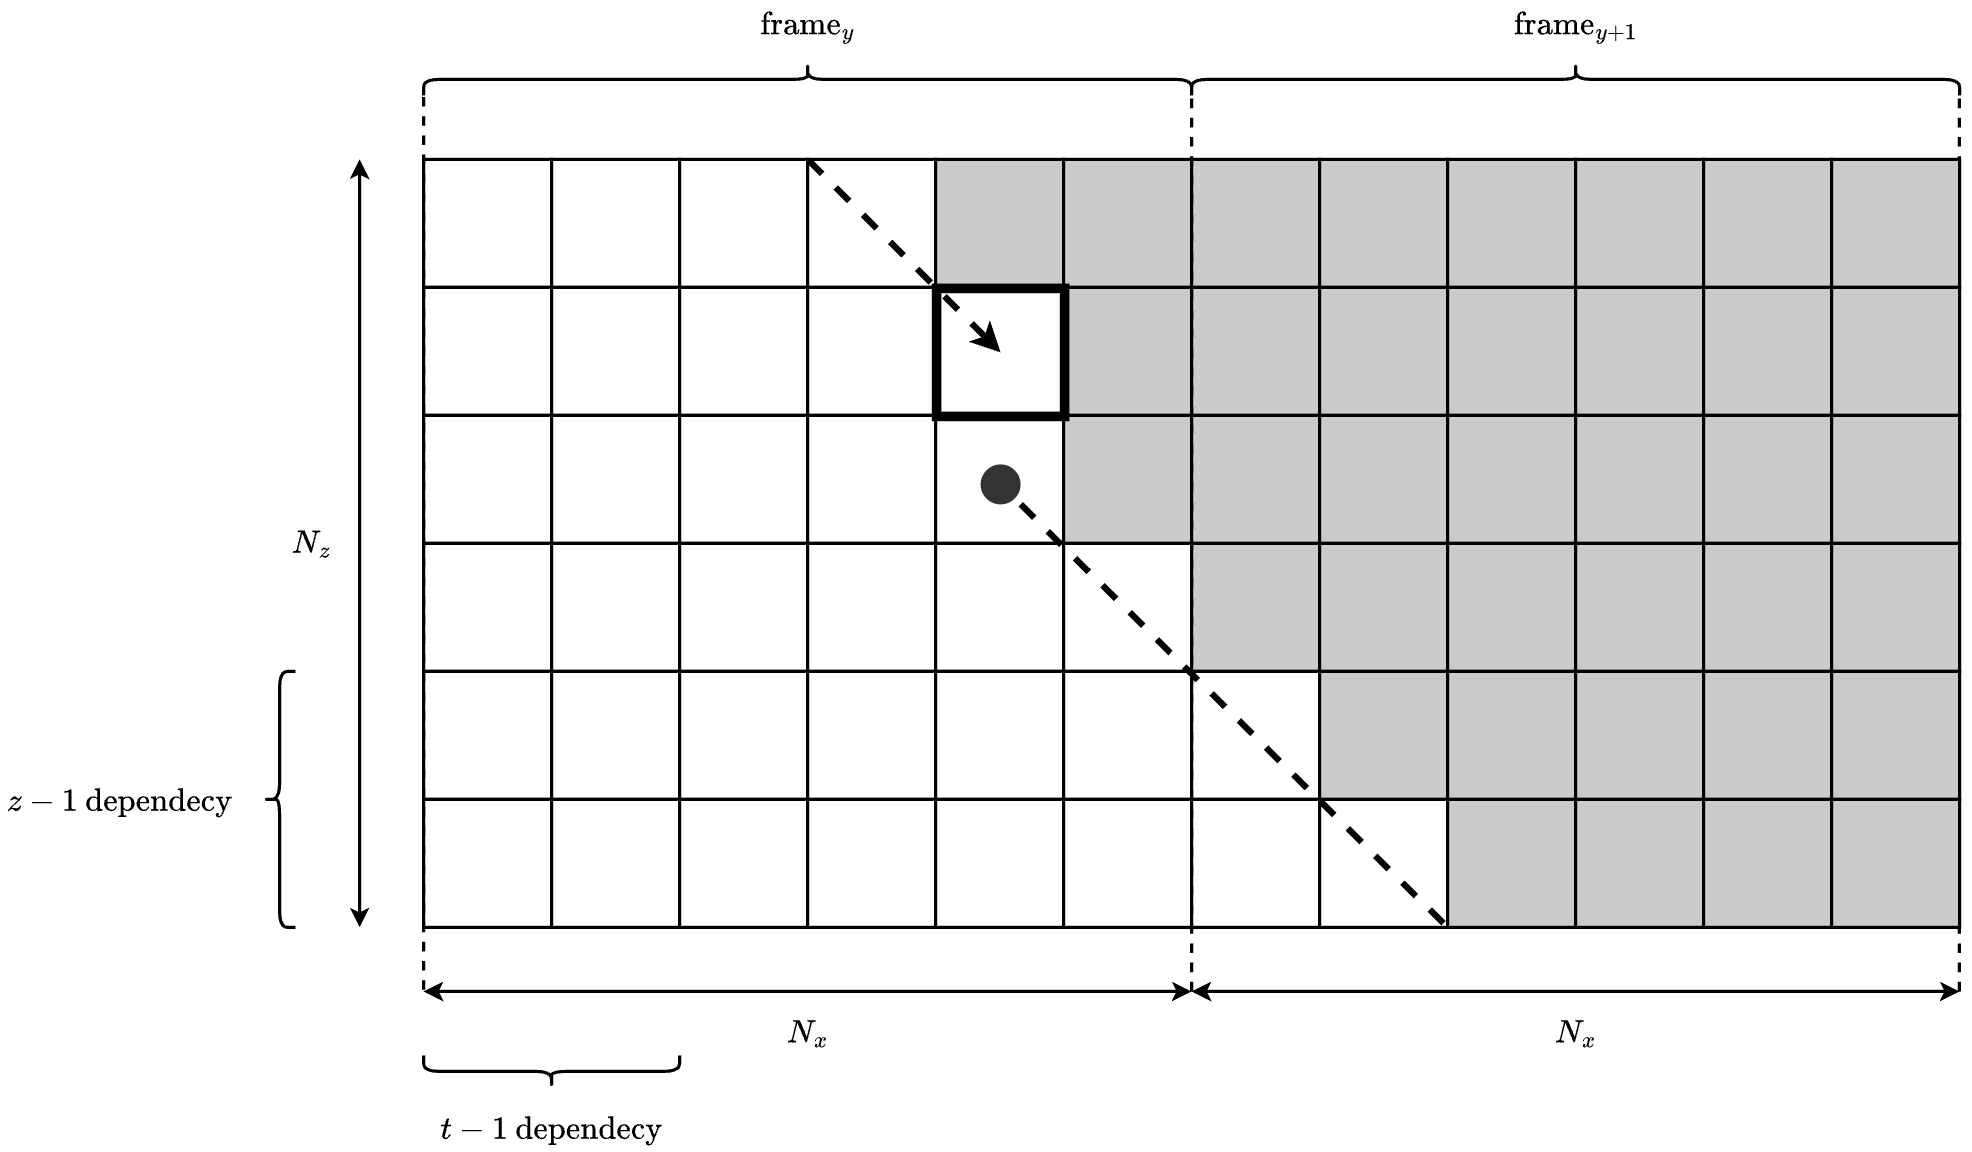
\includegraphics[width=1\textwidth]{figures/fid.png}
	\end{center}
	\caption{Novel \acrshort{FID} processing order presented by \citeauthor{basconesFPGAAcceleratorRealTime2020} interleaves all dependencies by a minimum of $N_z - 1$ samples, allowing deep pipelining.}
	\label{fig:fid}
\end{figure}

\begin{figure}[ht]
	\begin{center}
		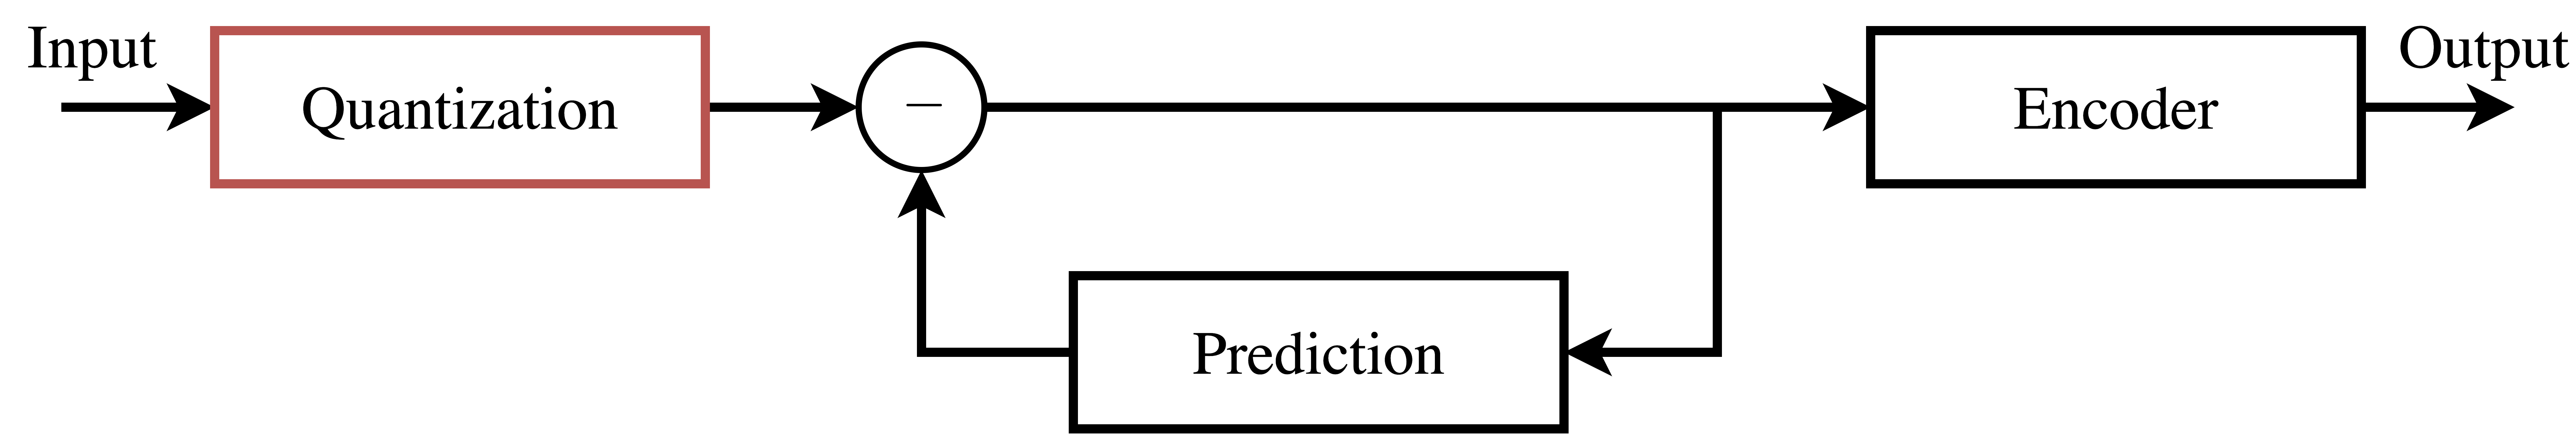
\includegraphics[width=0.9\textwidth]{figures/ccsds-prequantization.png}
	\end{center}
	\caption{Prequantization of image samples allows use of a lossless prediction loop, avoiding the challenging data dependencies.}
	\label{fig:prequantization}
\end{figure}

The works by \citeauthor{chatziantoniouScalableDataRateNearLossless2022a} and \citeauthor{valsesiaHighThroughputOnboardHyperspectral2019} suggest that the quantization step of the issue 2 predictor can be moved prior to the predictor as shown in \autoref{fig:prequantization} \cite{chatziantoniouScalableDataRateNearLossless2022a, valsesiaHighThroughputOnboardHyperspectral2019}. Image samples are quantized prior to prediction. This allows use of a lossless prediction loop, avoiding the need for sample representatives and the challenging data dependencies. The predictor can now be implemented using similar techniques as used by implementations of issue 1.

In addition to prequantization, \citeauthor{chatziantoniouScalableDataRateNearLossless2022a} employ image segmentation, a technique that may also be used by issue 2 compliant compressors as described in issue 2 green book \cite{LosslessMultispectralHyperspectral2022}. Reduction in compression performance is minimal for the segmented image, given that the segment sizes are large. Using VHDL \acrshort{RTL} and five cores, \citeauthor{chatziantoniouScalableDataRateNearLossless2022a} reach a throughput of 1375 MS/s, with a single core performance of 285 MS/s. This matches the results of \citeauthor{basconesRealTimeFPGAImplementation2022}, but at a larger area footprint.

Prequantization comes at a degradation in compression performance, both in terms of bitrate and image distortion, as opposed to the in-loop quantizer of issue 2. The works by \citeauthor{chatziantoniouScalableDataRateNearLossless2022a} and \citeauthor{valsesiaHighThroughputOnboardHyperspectral2019} show that the increase in bitrate and decreased image SNR are greatest for low bitrates. To combat this, \citeauthor{valsesiaHighThroughputOnboardHyperspectral2019} suggest using an on-ground computational neural network (CNN) to reconstruct lost data. During simulation, the method is able to mitigate data loss, and may be used for in-loop quantization as well as prequantization. However, the approach adds significant complexity to the reconstruction of images.

\begin{figure}[ht]
	\begin{center}
		
\includegraphics[width=1\textwidth]{figures/ccsds-pipeline-naive.png}
	\end{center}
	\caption{Suggested pipeline using reduced prediction mode, narrow local sums and \acrshort{BIL} processing order. Weight updates depend on results from the sample representative calculation, constraining the throughput.}
	\label{fig:ccsds-pipeline-naive}
\end{figure}

\citeauthor{sanchezReducingDataDependencies2022} identify that by using narrow local sums and reduced prediction mode, $t-1$ dependencies related to local sums and differences can be avoided (\autoref{fig:local-sums}) \cite{sanchezReducingDataDependencies2022}. Additionally, by using \acrshort{BIL} processing order, $z-1$ dependencies can be avoided (\autoref{tab:orderings-fid}). \autoref{fig:ccsds-pipeline-naive} shows a pipeline using these configuration. The weight update calculation, required by predicted central local differences, still has an unavoidable $t-1$ dependency, placing a significant restriction on the achievable throughput.

\citeauthor{barriosRemovingDataDependencies2024} present a solution in which the remaining data dependence of the weight updates is avoided by skipping weight updates entirely. This allows deep pipelining, but comes at the cost of reduced compression performance as the prediction loop can no longer dynamically adapt to image characteristics. To mitigate this, the authors use previous data sets to carefully select the initial weight values for specific image sensors. The analysis is based on compression for a set of absolute error limits, $\{0,1,3,7,15,31\}$, with performance penalties depending heavily on the image set. For some configurations the compress performance is even improved with up to $10\%$, but for most a worsening in the range $2-10\%$.

\citeauthor{sanchezReducingDataDependencies2022} also present a mathematically equivalent way of calculating the sign of the double-resolution prediction error $e_z(t)$, given by

\begin{equation}
	\text{sgn}^+\bigl[e_z(t)\bigr] =
	\begin{cases}
		-1,                                            & \text{if }\lvert s_z(t) - \hat{s}_z(t) \rvert \le m_z(t)\ \text{and }\tilde{s}_z(t)\text{ is odd},  \\[6pt]
		1,                                             & \text{if }\lvert s_z(t) - \hat{s}_z(t) \rvert \le m_z(t)\ \text{and }\tilde{s}_z(t)\text{ is even}, \\[6pt]
		\text{sgn}^+\bigl[s_z(t) - \hat{s}_z(t)\bigr], & \text{otherwise}.
	\end{cases}
	\label{eq:math-opt}
\end{equation}

This removes the dependence of the clipped quantizer bin center (\autoref{eq:double-resolution-prediction-error}), calculated in the samples representative stage, allowing calculation to start earlier (\autoref{fig:ccsds-pipeline-math-opt}). By speculatively calculating the weight updates for the two possible outcomes of the sign, weight updates may be calculated in parallel with the sign during the prediction stage. Once the sign calculation resolves, the correct outcome of the weight update is selected and passed to the predicted central local difference stage. This approach, dubbed the mathematical optimization approach, is evaluated by \citeauthor{barriosRemovingDataDependencies2024} using the \acrshort{HLS} methodology. Only the predictor module is evaluated, reaching a throughput of 231 MS/s. This is used as comparison for their approach of skipping weight updates, which reaches 236 MS/s. For both methods, only the predictor is implemented.

\begin{figure}[ht]
	\begin{center}
		\includegraphics[width=1\textwidth]{figures/ccsds-pipeline-math-opt.png}
	\end{center}
	\caption{Weight update dependence on sample representatives is alleviated using the mathematical optimization approach suggested by \citeauthor{sanchezReducingDataDependencies2022}. Speculative calculation of weight updates further increases throughput.}
	\label{fig:ccsds-pipeline-math-opt}
\end{figure}

The mathematical optimization approach is used by \citeauthor{vorhaugHyperspectralImageCompression2024} to develop a full issue 2 accelerator for use on-board the \acrshort{hypso} missions \cite{vorhaugHyperspectralImageCompression2024}. By use of VHDL \acrshort{RTL}, the design reaches a throughput of 110 MS/s on the Kintex XCKU040 \acrshort{FPGA}, the same \acrshort{FPGA} used in the evaluations of the previously mentioned issue 2 implementations. However, for the Zynq-7030, used on-board \acrshort{hypso}-1 and 2, a modest throughput of 67 MS/s is reached. This does not fulfill the real-time requirement of the \acrshort{hypso}-1 image sensor of 110.6 MS/s. The design is implemented without support for runtime configuration, resulting in the smallest compressor in open literature in terms of resource utilization.

\begin{figure}[ht]
	\begin{center}
		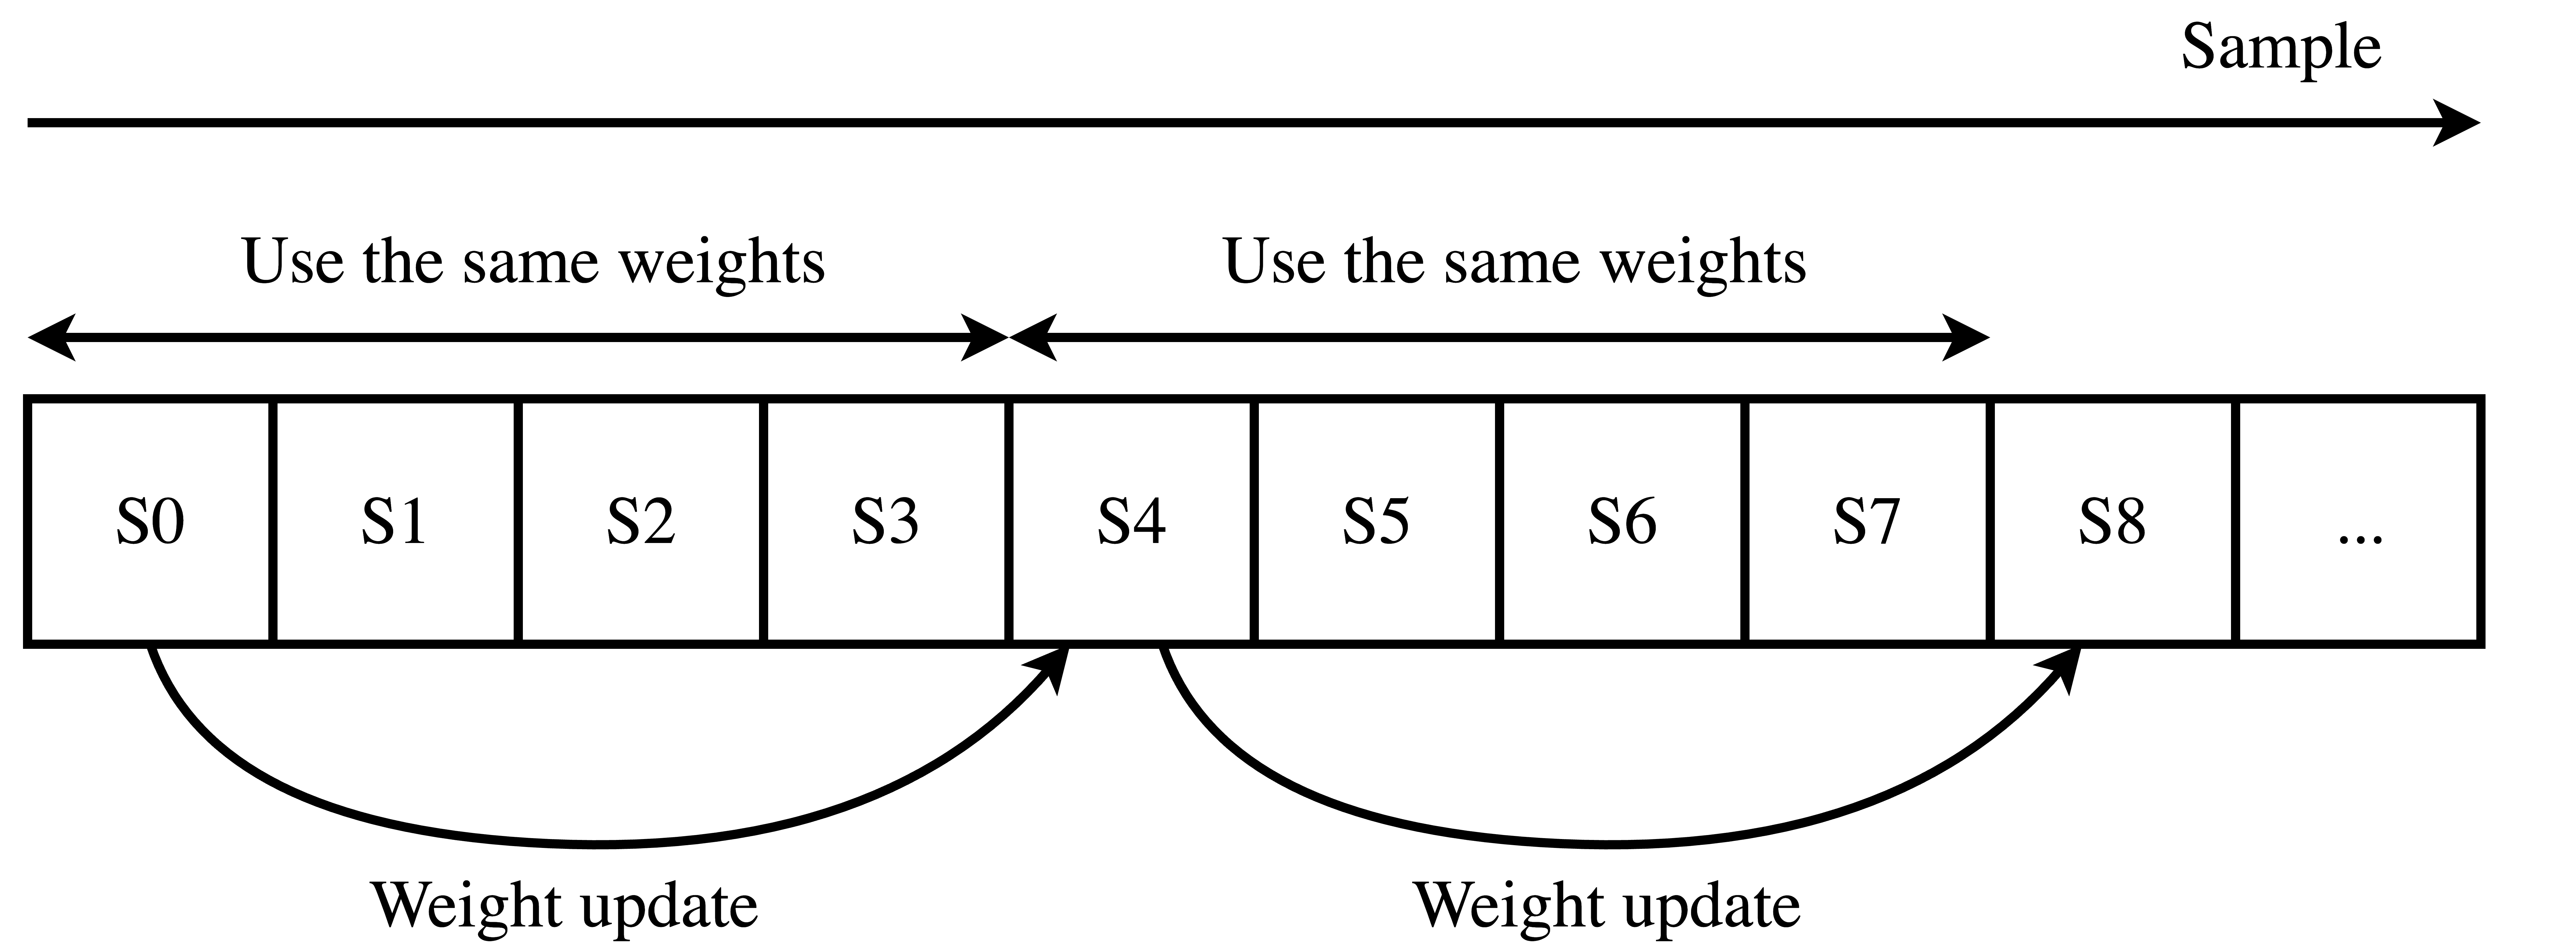
\includegraphics[width=0.8\textwidth]{figures/ccsds-weight-updates.png}
	\end{center}
	\caption{The proposed weight update scheme by \citeauthor{jiaRemovalFeedbackLoop2025}. Weights are kept unchanged for the first samples of every line, after which the sample from four samples earlier is used in the weight update calculation.}
	\label{fig:delayed-weight-updates}
\end{figure}

The achievable throughput of the mathematical optimization approach is constrained by the indivisible weight update calculation. To alleviate the problem, \citeauthor{jiaRemovalFeedbackLoop2025} suggest a modified weight update scheme, dubbed delayed weight updates \cite{jiaRemovalFeedbackLoop2025}. Their predictor is implemented using VHDL \acrshort{RTL}, reaching a throughput of 348 MS/s, while maintaining a small area footprint. Note that this result is achieved using a different \acrshort{FPGA}, Zynq XCZU5EV, than the previous works. Delayed weight updates come at slight degradation in compression performance. The analysis made by \citeauthor{jiaRemovalFeedbackLoop2025} is made using data sets from known missions, such as AVIRIS, over a set of absolute error limits, $\{0,1,3,7,15\}$. Results show a reduction in compression ratio in the range $1-5\%$, outperforming the approach of skipping weight updates as suggested by \citeauthor{barriosRemovingDataDependencies2024}.

\begin{equation}
	\omega^{(i)}_{z, \text{unclipped}}(t+1)=
	\begin{cases}
		\omega^{(i)}_z(t),                                                                                                                   & t \le 2,          \\[6pt]
		\omega^{(i)}_z(t-3) + \omega^{(i)}_{z, \text{offset}}(t-3),                                                                          & t = 3,            \\[6pt]
		\left\lfloor \dfrac{1}{2}\left(\omega^{(i)}_z(t-3) + \omega^{(i)}_{z, \text{offset}}(t-3) + \omega^{(i)}_z(t) \right) \right\rfloor, & \text{otherwise}.
	\end{cases}
	\label{eq:delayed-weight-updates}
\end{equation}

\begin{table}[ht]
	\caption{Hardware utilization and throughput of hardware accelerators of the issue 2 standard. The predictor module is the smallest and fastest in open litterature.}
	\label{tab:throughputs}
	\centering
	\begin{tabular}{l r r r r r r}
		\hline
		\textbf{Implementation}                                                                                      & \textbf{FPGA} & \textbf{LUT} & \textbf{FF} & \textbf{DSP} & \textbf{BRAM} & \textbf{Throughput} \\
		\hline
		Barrios et al.\ \cite{barriosHardwareImplementationCCSDS2021}                                                & XCKU040       & 17185        & 11915       & 63           & 85            & 18~MS/s             \\
		B\'ascones et al.\ \cite{basconesRealTimeFPGAImplementation2022}                                             & XQRKU060      & 16458        & 15707       & 30           & 187.5         & 285~MS/s            \\
		Chatziantoniou et al.\ \cite{chatziantoniouScalableDataRateNearLossless2022a} 1 core                         & XCKU040       & 18861        & 21395       & -            & 104           & 285~MS/s            \\
		Chatziantoniou et al.\ \cite{chatziantoniouScalableDataRateNearLossless2022a} 5 core                         & XCKU040       & 67362        & 68987       & -            & 306           & 1375~MS/s           \\
		S\'anchez et al.\ \cite{sanchezReducingDataDependencies2022, barriosRemovingDataDependencies2024}, predictor & XCKU040       & 19840        & 12970       & 33           & 213           & 231~MS/s            \\
		Barrios et al.\ \cite{barriosRemovingDataDependencies2024}, predictor                                        & XCKU040       & 11095        & 11729       & 20           & 186.5         & 236~MS/s            \\
		Vorhaug et al.\ \cite{vorhaugHyperspectralImageCompression2024}                                              & XCKU040       & 5577         & 2635        & 4            & 57.5          & 110~MS/s            \\
		Vorhaug et al.\ \cite{vorhaugHyperspectralImageCompression2024}                                              & XCZU7EV       & 5475         & 2635        & 4            & 57.5          & 141~MS/s            \\
		Jia et al.\ \cite{jiaRemovalFeedbackLoop2025}, predictor                                                     & XCZU5EV       & 3995         & 5050        & 7            & 94            & 348~MS/s            \\
		\hline
	\end{tabular}
\end{table}

